\documentclass[a4paper,14pt]{extreport}
\usepackage[T2A]{fontenc}
\usepackage[utf8x]{inputenc}%включаем свою кодировку: koi8-r или utf8 в UNIX, cp1251 в Windows
\usepackage[russian]{babel}%используем русский и английский языки с переносами
\usepackage{indentfirst}
\usepackage{cite,enumerate,float}
\usepackage{amsmath, amssymb}
\usepackage{fancyvrb}
\usepackage{graphicx}
\graphicspath{{images/},{plots/}}%путь к рисункам

\usepackage{multicol, multirow, array}
\newcolumntype{C}[1]{>{\centering\arraybackslash}m{#1\textwidth}}
\renewcommand{\arraystretch}{1.2}


\usepackage{geometry}
\geometry{left=3cm}% левое поле
\geometry{right=1.5cm}% правое поле
\geometry{top=2cm}% верхнее поле
\geometry{bottom=2cm}% нижнее поле

\usepackage{tocloft}
\renewcommand{\cfttoctitlefont}{\normalfont}
\makeatletter
\renewcommand*\l@chapter[2]{%
  \ifnum \c@tocdepth >\z@
    \addpenalty\@secpenalty
    \addvspace{0.5em \@plus\p@}%
    \setlength\@tempdima{1.5em}%
    \begingroup
      \parindent \z@ \rightskip \@pnumwidth
      \parfillskip -\@pnumwidth
      \leavevmode
      \advance\leftskip\@tempdima
      \hskip -\leftskip
      #1\nobreak\cftdotfill{\cftdotsep} \nobreak\hb@xt@\@pnumwidth{\hss #2}\par
    \endgroup
  \fi}
\renewcommand*\l@section[2]{%
  \ifnum \c@tocdepth >\@ne
    \addpenalty\@secpenalty
    \addvspace{0.5em \@plus\p@}%
    \setlength\@tempdima{1.5em}%
    \begingroup
      \parindent \z@ \rightskip \@pnumwidth
      \parfillskip -\@pnumwidth
      \leavevmode
      \advance\leftskip\@tempdima
      \hskip -\leftskip
      #1\nobreak\cftdotfill{\cftdotsep} \nobreak\hb@xt@\@pnumwidth{\hss #2}\par
    \endgroup
  \fi}
\renewcommand*\l@subsection[2]{%
\ifnum \c@tocdepth >\tw@
  \addpenalty\@secpenalty
  \addvspace{0.5em \@plus\p@}%
  \setlength\@tempdima{1.5em}%
  \begingroup
    \parindent \z@ \rightskip \@pnumwidth
    \parfillskip -\@pnumwidth
    \leavevmode
    \advance\leftskip\@tempdima
    \hskip -\leftskip
    #1\nobreak\cftdotfill{\cftdotsep} \nobreak\hb@xt@\@pnumwidth{\hss #2}\par
  \endgroup
\fi}
\makeatother
\usepackage{setspace}

\usepackage{titlesec}
\usepackage[square, numbers, sort&compress]{natbib}
\usepackage[unicode, colorlinks, linkcolor=black,
citecolor=black,urlcolor=black]{hyperref}

\renewcommand{\arraystretch}{1.2}

\renewcommand{\small}{\fontsize{12pt}{14.4pt}\selectfont}
\usepackage{caption}
\DeclareCaptionLabelFormat{figure}{Рисунок #2}
\DeclareCaptionLabelFormat{table}{Таблица #2}
\DeclareCaptionLabelSeparator{sep}{~---~}
\captionsetup{labelsep=sep,justification=centering,font=small}
\captionsetup[figure]{labelformat=figure}
\captionsetup[table]{labelformat=table}

\renewcommand{\theenumi}{\arabic{enumi}}
\renewcommand{\labelenumi}{\arabic{enumi})}
\renewcommand{\theenumii}{.\arabic{enumii}}
\renewcommand{\labelenumii}{\arabic{enumi}.\arabic{enumii})}
\renewcommand{\theenumiii}{.\arabic{enumiii}}
\renewcommand{\labelenumiii}{\arabic{enumi}.\arabic{enumii}.\arabic{enumiii})}

\newcommand{\pder}[2] {\frac{\partial #1}{\partial #2}}
      % частная производная от #1 по #2
\newcommand{\ppder}[2]{\frac{\partial^2 #1}{\partial {#2}^2}}
  % вторая частная производная от #1 по #2
\newcommand{\pcder}[3]{\frac{\partial^2 #1}{\partial #2 \partial #3}}
  % вторая частная производная от #1 по #2 и #3
\newcommand{\der}[2]  {\frac{d #1}{d #2}}
  % производная от #1 по #2
\newcommand{\dder}[2] {\frac{d^2 #1}{d {#2}^2}}
  % вторая производная от #1 по #2

% --- обозначения и команды ---
\newcommand{\const}{\mathrm{const}}                     % константа
\newcommand{\average}[1]{\left\langle #1 \right\rangle} % обозначение среднего
\newcommand{\abs}[1]{\left| #1 \right|}                 % обозначение модуля
\newcommand{\ds}{\displaystyle}                         % полный размер строчной формулы
\newcommand{\D}{\Delta}
\newcommand{\dotunder}[1]{\d{#1}} % необходима для обозначения строчной дельты
\renewcommand{\d}{\delta}
\newcommand{\eps}{\varepsilon}
\renewcommand{\phi}{\varphi}
% xxx обозначения и команды xxx

\newcommand{\divergence}{\mathrm{div\,}}  % дивергенция
\newcommand{\gradient}  {\mathrm{grad\,}} % градиент
\newcommand{\rotor}     {\mathrm{rot\,}}  %
\renewcommand{\vec}[1]{\boldsymbol{#1}}
% title style
\titleformat{\chapter}
    {\centering\normalsize}
    {\thechapter}
    {8pt}{\MakeUppercase}
\titleformat{\section}
    {\centering\normalsize}
    {\thesection}
    {1em}{}
\titleformat{\subsection}
    {\centering\normalsize}
    {\thesubsection}
    {1em}{}

\titlespacing*{\chapter}{0pt}{-30pt}{8pt}
\titlespacing*{\paragraph}{0pt}{-30pt}{8pt}
\titlespacing*{\section}{\parindent}{*4}{*4}
\titlespacing*{\subsection}{\parindent}{*4}{*4}

\makeatletter

\renewcommand{\@biblabel}[1]{#1}

% bibliography bibitem item indent
\renewenvironment{thebibliography}[1]
    {\chapter*{\bibname}%
    \@mkboth{\MakeUppercase\bibname}{\MakeUppercase\bibname}%
    \list{\@biblabel{\@arabic\c@enumiv}}%
        {\settowidth\labelwidth{\@biblabel{#1}}%
        \leftmargin=0pt
        \itemindent=50pt
        \@openbib@code
        \usecounter{enumiv}%
        \let\p@enumiv\@empty
        \renewcommand\theenumiv{\@arabic\c@enumiv}}%
    \sloppy
    \clubpenalty4000
    \@clubpenalty \clubpenalty
    \widowpenalty4000%
    \sfcode`\.\@m}
        {\def\@noitemerr
        {\@latex@warning{Empty `thebibliography' environment}}%
    \endlist}

\makeatother

\newcolumntype{C}[1]{>{\centering\arraybackslash}m{#1\textwidth}}
\renewcommand{\arraystretch}{1.2}

\DeclareCaptionLabelFormat{figure}{Рисунок #2}
\DeclareCaptionLabelFormat{table}{Таблица #2}
\DeclareCaptionLabelSeparator{sep}{~---~}
\captionsetup{labelsep=sep, justification=centering, font=small}
\captionsetup[figure]{labelformat=figure}
\captionsetup[table]{labelformat=table}

\renewcommand{\cftloftitlefont}{\normalfont\hspace{0.38\textwidth}}
\renewcommand{\cftlottitlefont}{\normalfont\hspace{0.38\textwidth}}
\renewcommand{\cfttoctitlefont}{\normalfont\hspace{0.38\textwidth}}
\renewcommand{\cftbeforetoctitleskip}{-1em}

\renewcommand{\cftchapfont}{\normalsize}
\renewcommand{\cftsecfont}{\hspace{-21pt}}
\renewcommand{\cftsubsecfont}{\hspace{-53pt}}
\renewcommand{\cftbeforechapskip}{0em}
\renewcommand{\cftparskip}{-1mm}
\renewcommand{\cftdotsep}{1}
\renewcommand{\cftsecpresnum}{}
\renewcommand{\cftchapleader}{\cftdotfill{\cftdotsep}}
\renewcommand{\cftsecleader}{\cftdotfill{\cftdotsep}}
\renewcommand{\cftsecaftersnum}{.}
\renewcommand{\cftsubsecaftersnum}{.}
\setcounter{tocdepth}{2}

\renewcommand{\theenumi}{\arabic{enumi}}
\renewcommand{\labelenumi}{\arabic{enumi})}
\renewcommand{\theenumii}{.\arabic{enumii}}
\renewcommand{\labelenumii}{\arabic{enumi}.\arabic{enumii})}
\renewcommand{\theenumiii}{.\arabic{enumiii}}
\renewcommand{\labelenumiii}{\arabic{enumi}.\arabic{enumii}.\arabic{enumiii})}
\tolerance=10000
\begin{document}
  \onehalfspacing
  \setlength{\parindent}{1.25cm}
  \begin{titlepage}
    \begin{center}
        Государственное бюджетное образовательное учреждение высшего
        профессионального образования\\
        «Волгоградский государственный технический университет»\\
        \vspace{1em}
        Факультет электроники  и  вычислительной  техники\\
        \vspace{0.6em}
        Кафедра физики\\ 
    \end{center}
    \begin{flushright}
        УТВЕРЖДАЮ\\
        \vspace{0.6em}
        \parbox{7cm}{
        Научный руководитель профиля \\
        магистерского направления\\
        д.ф.-м.н., профессор}\\
        \vspace{1em}
        \rule[-0.05cm]{4.5cm}{.1pt} Шеин~А.~Г.\\
        <<\rule[-0.05cm]{1cm}{.1pt}>>\rule[-0.05cm]{4cm}{.1pt} 2014 г.
    \end{flushright}
    \vfill
    \begin{center}
        ОТЧЕТ\\
        О  НАУЧНО-ИССЛЕДОВАТЕЛЬСКОЙ РАБОТЕ\\
        \vspace{1em}
        Энергетический спектр муаровых сверхрешёток на основе графена
        (промежуточный, 1 семестр)
    \end{center}
    Студент группы Ф-1н Абдрахманов Владимир Леватович \hfill \rule[-0.05cm]{3.5cm}{.1pt}
    \vspace{1em}
    \begin{flushright}
    Научный руководитель магистерской диссертации \hfill ~\\
        д.~ф.-м.~н.,~проф.,~Завьялов~Д.~В.
    \end{flushright}
    \vfill
    \begin{center}
        Волгоград 2014
    \end{center}
\end{titlepage}
\setcounter{page}{2}
  \begin{center}
    РЕФЕРАТ
\end{center}

В работе сделан краткий обзор основ теории функционала плотности, на которой основаны современные пакеты квантовой химии. Рассмотрены три таких пакета: ABINIT, QUANTUM ESPRESSO и CRYSTAL. С их помощью произведён расчёт зонной структуры бесконечного листа графена. Проведено сравнение полученных результатов.

\vspace{1cm}
\noindent Ключевые слова: ТФП, графен, зонная структура, конус Дирака, ABINIT, CRYSTAL, QUANTUM ESPRESSO

\vspace{2cm}
\begin{center}
    ABSTRACT
\end{center}

In this paper brief overview of the basics of density functional theory, which  modern quantum chemistry packages is based on, is given. Consider three packages: ABINIT, QUANTUM ESPRESSO and CRYSTAL. With their help, the calculation of the band structure of an infinite graphene sheet were promoted. The results are compared.

\vspace{1cm}
\noindent Keywords: DFT, graphene, band structure, Dirac cone, ABINIT, CRYSTAL, QUANTUM ESPRESSO
  \newpage
  \renewcommand{\contentsname}{\begin{center}СОДЕРЖАНИЕ\end{center}}
  \tableofcontents
  \newpage
  \begin{center}
    Введение
\end{center}
\addcontentsline{toc}{chapter}{Введение}

Для изучения особенностей зонной структуры твёрдых тел в современной теоретической физике используются различные квантовохимические пакеты. Многие из них основаны на методах DFT --- теории функционала плотности (ТФП), разработанной в 60-x годах прошлого века. Для проведения расчётов в моей магистерской работе следует ознакомиться с некоторыми из таких пакетов, научиться задавать в них конфигурацию исследуемой системы и извлекать необходимые результаты, полученные в результате работы. 

В этой работе рассмотрены 3 пакета: свободные ABINIT и QUANTUM ESPRESSO, а также проприетарный CRYSTAL (демонстрационная версия).

  \chapter{Теория функционала плотности}
Одна из самых главных проблем теоретической химии твердого тела состоит в разработке соответствующих методов для решения многоэлектронного уравнения Шредингера. Метод Хартри-Фока обеспечивает приближенное решение для задачи N частиц, но не подходит для больших систем. Наиболее часто используемыми методами являются методы на основе теории функционала плотности (DFT).

Теория функционала плотности (DFT) , cформулированная Хоэнбергом и Коном (HK) и разработанная Коном и Шэмом (KS), основана на том, что энергия основного состояния системы является фнкционалом электронной плотности \(\rho(\vec{r})\).
Волновая функция системы из \(N\) электронов содержит \(3N\) координат, по три для каждого электрона. Электронная плотность \(\rho(\vec{r})\) является квадратом волновой функции, интегрированной по координатам \(N-1\) электронов: \(\rho(\vec{r})\) зависит только от трех координат, независимо от числа электронов. Это означает, что, в то время как сложность волновой функции возрастает с увеличением числа электронов, плотность электронов имеет одинаковое число переменных, независимо от размера системы.

ТФП основана на двух теоремах. Первая теорема HK утверждает все электронные свойства системы в основном состоянии определяются электронной плотностью основного состояния.

Вторая теорема HK связывает основное состояние электронной плотности \(\rho_0(\vec{r})\) системы с ее полной энергией:
\begin{equation}
    E[\rho(\vec{r})] \ge E[\rho_0(\vec{r})] \cong E.
\end{equation}
Полная энергия:
\begin{equation}
    E[\rho(\vec{r})] = T[\rho(\vec{r})] + V_{ee}[\rho(\vec{r})]+
    \int\limits_D \rho(\vec{r}) v(\vec{r}) d\vec{r},
    \label{eq:36}
\end{equation}
где \(T\) кинетическая энергия электронов, \(V_{ee}\) -- электрон-электронный вклад и \(v(\vec{r}\) является потенциалом, действующим на электроны, включающим в себя ядерно-электронного взаимодействия и внешний потенциал, действующей на систему. Так как выражения для \( T \) и \(V_{ee}\) точно известны, основное состояние может быть определено путем непосредственного минимизации функционала \eqref{36}.

Метод Кона-Шема состоит в принятии в качестве отсчёта не взаимодействующей электронной системы, для которой кинетическая энергия может быть вычислена. Электрон-электронные взаимодействия, следовательно, могут быть рассчитаны в классическом  приближении усредненного поля, в то время как все неклассические вклады (корреляции) в Ve и вклад невзаимодействующих электронов в кинетическую энергию включены в корреляционно-обменный член:
\begin{equation}
    E_{xc}[\rho(\vec{r})] = V_{ee} - \frac{1}{2}\int\limits_{D}\frac{\rho(\vec{r})\rho(\vec{r}')}{|\vec{r} - \vec{r}'|}.
    \label{eq:37}
\end{equation}

\( \rho(\vec{r}) \)  может быть выражено в терминах одноэлектронных функций \( \psi_i \):
\begin{equation}
    \rho(\vec{r}) = \sum_{i=1}^N |\psi_i|^2,
\end{equation}
где \(\psi_i\) являются решениями \( N \) одноэлектронных уравнений Кона-Шэма
\begin{gather}
    \hat{H}\psi_i = \eps_i\psi_i,\quad i=1,\ldots,N\\
    \hat{H} = \hat{T} + \hat{Z} + \hat{C} + \hat{E}_{xc}.
\end{gather}
Таким образом, в отличие от метода Хартри-Фока в ТФП учитывается корреляционная энергия. Функционал Exc определяется следующим образом:
\begin{equation}
    E_{xc} = \pder{E_{xc}[\rho(\vec{r})]}{\rho(\vec{r})}
\end{equation}
Если обмено-корреляционный член известен, уравнения KS обеспечивают точные решения. Для того, чтобы применить метод ТФП, однако, приблизить формулировки Ехс должны быть определены: различия между ТФП методов в выборе его функционального вида. Простейшим решением является приближение локальной плотности (LDA):
\begin{equation}
    E_{xc}^{LDA}[\rho(\vec{r})] = \int\limits_{D}\eps_{xc}(\rho(\vec{r}))\rho(\vec{r}) d\vec{r},
\end{equation}
где \(\eps_{xc}(\rho(\vec{r}))\) является обменно-корреляционной энергии для частицы в однородном электронно-взаимодействующий газ с плотностью \(\rho(\vec{r})\).

Более точное приближение -- обобщённое градиентное приближение (GGA)
\begin{equation}
    E_{xc}^{GGA}[\rho(\vec{r})] = \int\limits_{D}f(\rho(\vec{r}), \nabla\rho(\vec{r})) d\vec{r},
\end{equation}
где \( f(\rho(\vec{r}), \nabla\rho(\vec{r})) \) является функцией как электронной плотности и её градиента. GGA позволяет лучше описывать неоднородные системы.

Наиболее часто используются комбинации функционалов с привлечением точного результата, полученного методом Хартри — Фока, так как они, как правило, обеспечивают большую точность в оптимизации геометрии, энергетических расчетов. Они известны как гибридные методы.
  \chapter{Квантово-химические пакеты}
\section{ABINIT}
ABINIT основывается на теории функционала плотности (ТФП). Для функций отклика, таких как вибрации, диэлектрические или пьезоэлектрические свойства, реализована специализированная версия ТФП, теория возмущений функционала плотности, обеспечивающая эффективность и простоту использования. Основные возможности ABINIT реализуются с помощью этих двух методов ТФП. Тем не менее, для расчёта электронных свойств, в частности, ширины запрещенной зоны, методы теории функционала плотности, как известно, ненадежны. В ABINIT, такие электронные свойства могут быть вычислены точно благодаря реализации многочастичной теории возмущений, так называемого <<GW приближения>>.

В программе реализованы различные приближения функционала обменно-корреляционной энергии, в том числе различных видов приближении локальной плотности и обобщенного градиентного приближения. С помощью этих приближений, длины связей и углы, как правило, предсказываются с точностью в пределах нескольких процентов.

ABINIT основан на разложении электронных волновых функций на плоские волны, с периодическим представлением системы в ящике при периодических граничных условиях. Это представление особенно подходит для исследования кристаллов: ящик принимается в качестве примитивной элементарной ячейки. Если принимать непримитивную ячейку (или сверх-ячейку), то можно изучать системы, в которых трансляционная симметрия отсутствует. Чтобы дать некоторое представление о размерах разрешенных систем, отметим, что для тестирования ABINIT были использованы системы, содержащие до 250 атомов, в то время как в большинстве ТФП расчётов ABINIT размер ячейки не превышает 50 атомов, и даже, в случае более требовательного GW исследования, число атомов не достигает и десятка.

Псевдопотенциалы позволяют не рассматривать внутренние электроны и сосредоточить внимание на формировании связей и свойствах валентных электронов. ABINIT имеет обширную библиотеку псевдопотенциалов для всей таблицы Менделеева.

С помощью ABINIT достаточно просто изучать как металлы, так и диэлектрики: сетки волновых векторов, необходимые для расчёта вклада каждого электрона в зоне Бриллюэна создаются автоматически. Для металлов, различные схемы размытия позволяют уменьшить количество таких волновых векторов.

Основным результатом ТФП является электронная плотность. В ABINIT, из-за использования псевдопотенциалов рассматриваются плотности валентных электронов. 

Как уже упоминалось, использование ТФП для расчёта зонной структуры находится под вопросом, и, следовательно, должно быть ограничено качественным анализом. Это особенно важно при исследовании вещества на металлические или диэлектрические свойства или количественном расчёте ширины запрещенной зоны.

Методология GW, наоборот, как правило, позволяет достичь очень хорошего описания зонной структуры и запрещенных зон, с погрешностью менее 0,2 эВ по отношению к экспериментальным данным. Расчет GW выполняется для заданной геометрии (оптимизированной или экспериментальной), после выполнения расчета ТФП (необходимы электронные волновые функции).\cite{abinit}

  \section{QUANTUM ESPRESSO}
QUANTUM ESPRESSO реализует различные методы и алгоритмы, направленные на химически реалистичное моделирование материалов, начиная с наноразмерных, на основе решения задачи теории функционала плотности (DFT) с использованием базиса плоских волн и псевдопотенциалов, чтобы представить электрон-ионные взаимодействия.

Программа построена на использовании периодических граничных условий, что позволяет просто рассчитывать бесконечные кристаллические системы. Конечные системы рассчитываются с помощью сверхячеек. QUANTUM ESPRESSO таким образом, может быть использован для любой кристаллической структуры или сверхячейки как металлов, так и диэлектриков. Атомные ядра могут быть описаны различными наборами волн. Имеется множество различных обменно-корреляционных функционалов локальной плотности (LDA) или обобщенного градиентного приближений (GGA), а также такие функционалы, как U-поправки Хаббарда, несколько мета-GGA и гибридные функционалы.

Ниже представлен неполный список расчетов, которые могут быть выполнены при помощи программы \cite{qe}:
\begin{itemize}
    \item расчет Кона-Шэма (KS) орбиталей и энергий для изолированных или периодических систем, и их энергий основного состояния;
    \item полные структурные оптимизации микроскопических (атомные координаты) и макроскопических (ячейки) степеней свободы, используя силы и напряжения Гельмана-Фейнмана;
    \item расчёт основного состояния магнитных или спин-поляризованных систем, в том числе спин-орбитального взаимодействия и неколлинеарного магнетизма;
    \item теория возмущений функционала плотности (DFPT);
    \item получение максимально локализованных функций Ванье и связанных с ними величин;
    \item расчет параметров ядерного магнитного резонанса (ЯМР) и электронного парамагнитного резонанса (ЭПР);
    \item расчет К-края спектров рентгеновского поглощения.
\end{itemize}

  \section{CRYSTAL}
Пакет CRYSTAL выполняет первопринципные расчеты энергии основного состояния, градиента энергии, электронной волновой функции и свойств периодических систем. Могут быть использованы гамильтонианы Хартри-Фока или Кона-Шэма. На равных основаниях рассматриваются периодические системы в 0 (молекулы, 0D), 1 (полимеры, 1D), 2 (листы, 2D) и 3-х измерениях (кристаллы, 3D). В каждом случае в качестве приближения используется разложение волновых функций одной частицы (CO) в виде линейной комбинации функций Блоха (BF) определённых с помощью локальных функций (АО).

Локальные функции, в свою очередь, представляют из себя линейные комбинации функций гауссового типа (GTF), показатели и коэффициенты которых определяются входными данными. Могут быть использованы функции симметрии s, p, d и f. Также доступны sp-оболочки (s- и р-оболочки с общим набором показателей). Использование sp оболочек может привести к значительной экономии процессорного времени.

Программа может автоматически обрабатывать пространственные симметрии: 230 пространственных групп, 80 групп слоев, 99 одномерных группы, 45 точечные группы. Точечные симметрии, совместимые с трансляционной симметрией, предназначены для молекул.

Программа позволяет создавать специальные 1D (нанотрубки) и 0D (фуллерены) структуры из 2D структур, а также генерировать листы (2D системы) или кластеры (система 0D) из 3D-кристаллической структуры, упругие деформации решетки, создавать сверх-ячейки с дефектом и разнообразно редактировать структуры.\cite{crystal}
  \chapter{Графен}
Для ознакомления с перечисленными выше пакетами в качестве примера использовался лист графена. Выбор обусловлен тем, что с одной стороны это основа сверхрешёток, которые будут изучаться в дальнейшем, а с другой стороны в литературе представлена зонная структура графена и полученные в ходе работы программы результаты есть с чем сравнивать.

\begin{figure}[h]
    \center
    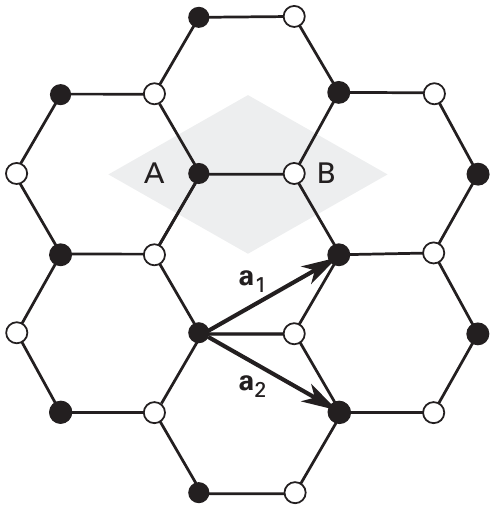
\includegraphics[width=.4\textwidth]{gra}\hfill
    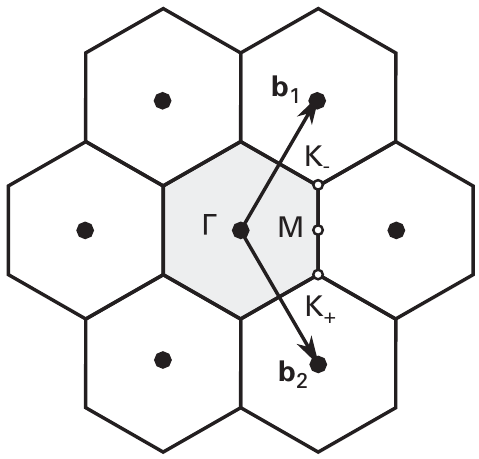
\includegraphics[width=.4\textwidth]{grb}
    \parbox[t]{.4\textwidth}{\center а)}\hfill
    \parbox[t]{.4\textwidth}{\center б)}
    \caption{Прямая (а) и обратная (б) решётки графена}
    \label{graphene}
\end{figure}

Графен представляет из себя двухмерный кристалл, в узлах кристаллической решётки которого располагаются атомы углерода. Он обладает гексагональной решёткой, в элементарной ячейке которой находятся 2 атома (рисунок~\ref{graphene}а). Обратная решётка также гексагональна, поэтому зона Бриллюэна имеет форму шестиугольника (рисунок~\ref{graphene}б).

Характерной особенностью зонной структуры графена является так называемый конус Дирака. В углах шестиугольной зоны Бриллюэна (в точках K) зона проводимости пересекается с валентной зоной, причём закон дисперсии вблизи этих точек линеен. Поэтому вблизи них поверхность \(E(\vec{k})\) представляет собой конус. Вершина этого конуса располагается на уровне Ферми.
  \chapter{Результаты}
 
 Для ознакомления с программами мною были составлены входные файлы для всех трёх вышеупомянутых пакетов, рассчитывающие зонную структуру однородного бесконечного листа графена методами DFT. Использованные входные файлы для программ представлены в приложениях А Б и В. Также для обработки данных и визуализации зонной структуры мной был написан скрипт, представленый в приложении Г.

 Полученные результаты представлены на рисунке~\ref{bands}а.
\begin{figure}[h]
    \center
    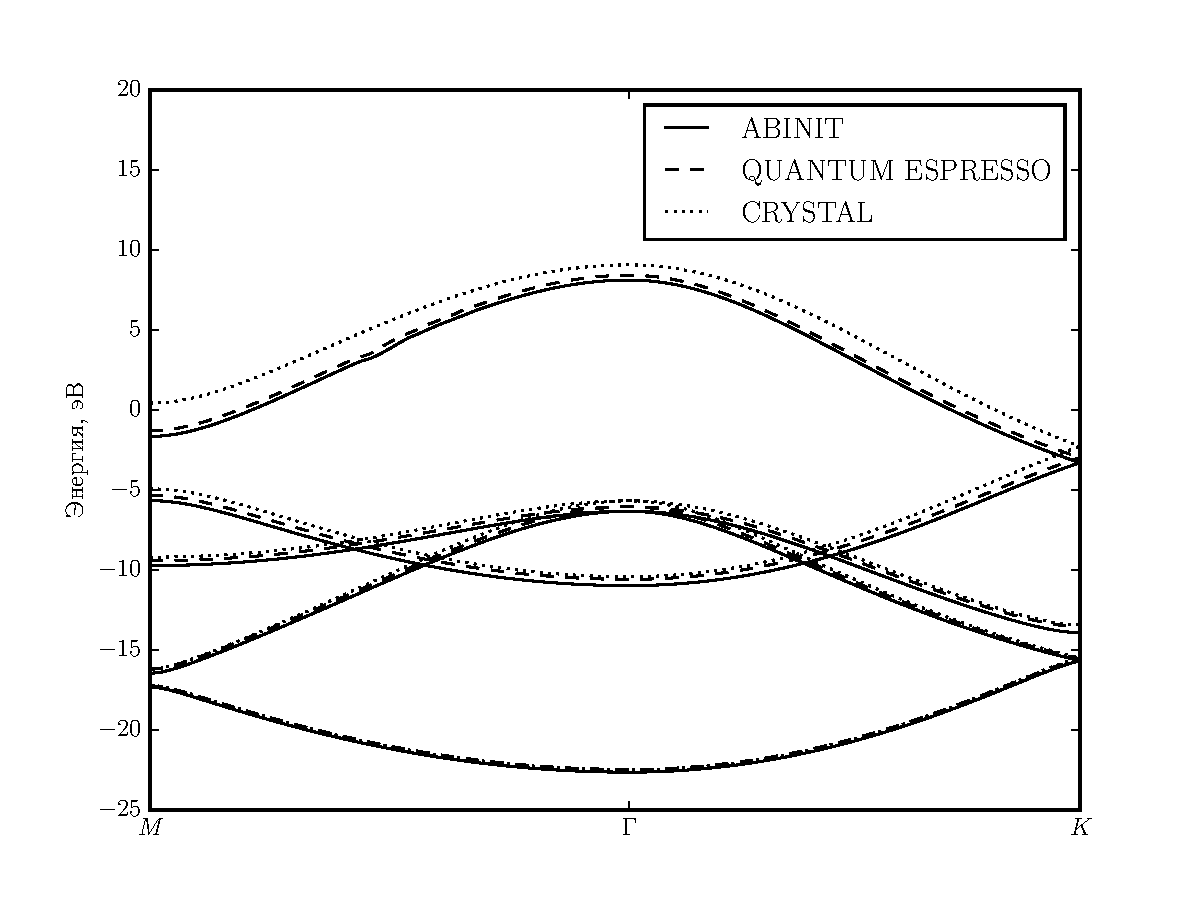
\includegraphics[width=.47\textwidth]{res}\hfill
    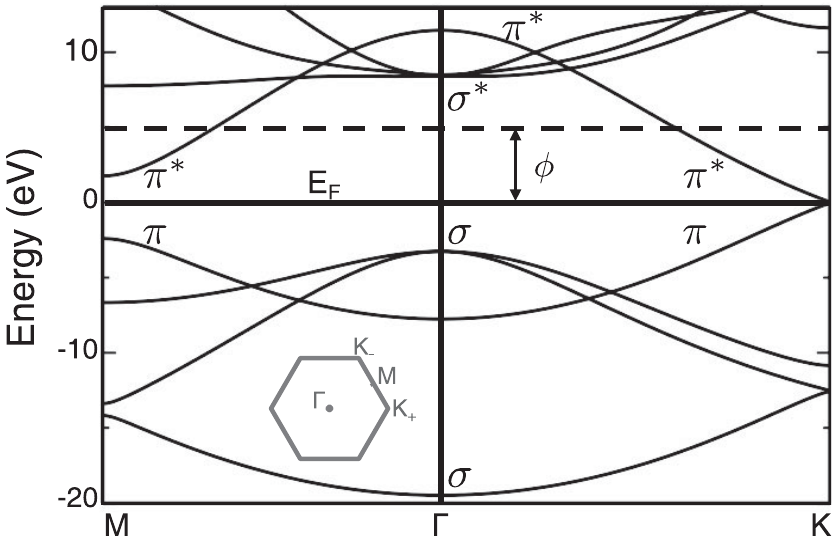
\includegraphics[width=.47\textwidth]{lit}
    \parbox[t]{.47\textwidth}{\center а)}\hfill
    \parbox[t]{.47\textwidth}{\center б)}
    \caption{Зонная структура графена: по результатам расчётов (а) и представленная в \cite{graphene} (б)}
    \label{bands}
\end{figure}
 Из представленных графиков видно, что все три программы дают качественно правильные результаты. На всех трёх зонных структурах для двух верхних зон вблизи точки K наблюдается участок с линейной дисперсией -- конус Дирака. ABINIT и QUANTUM ESPRESSO дают почти идентичные результаты. Для нижних зон результаты совпадают, а для верхних расхождение составляет не более 0,3 эВ. Результаты CRYSTAL так же совпадают с другими на нижних зонах, но на верхних разница с двумя другими пакетами составляет более 1 эВ.

 В книге \cite{graphene} представлена иллюстрация зонной структуры графена изображённая на рисунке~\ref{bands}б. Результаты, полученные с помощью ABINIT и QUANTUM ESPRESSO, хорошо соотносятся, с результатами, представленными на этом графике. CRYSTAL даёт завышенную энергию \( \pi \)-зон.
  \newpage
  \begin{center}
    ЗАКЛЮЧЕНИЕ
\end{center}
\addcontentsline{toc}{chapter}{Заключение}

В данной работе были рассмотрены 3 пакета квантовохимических вычислений, с их помощью была получена зонная структура листа графена. Два из них, ABINIT и QUANTUM ESPRESSO, продемонстрировали схожие с экспериментальными данными результаты, в то время как результаты CRYSTAL отличались большей погрешностью. Учитывая этот факт, а так же то, что первые два из трёх рассмотренных пакетов бесплатные, для проведения дальнейших расчётов стоит отдать предпочтение одному из них, используя другой для проверки результатов.

  \newpage
  \addcontentsline{toc}{chapter}{Список использованных источников}
\def\bibname{СПИСОК ИСПОЛЬЗОВАННЫХ ИСТОЧНИКОВ}
\begin{thebibliography}{99}
\bibitem{dft} \textbf{Eschrig, H.} The Fundamentals of Density Functional Theory (revised and extended version) [Electronic resource]~/ H. Eschrig.~--- Mode of access: \url{https://www.ifw-dresden.de/userfiles/groups/itf\_folder/Helmut_Eschrig/dft.pdf}.~--- Date of access: 22.12.2014.
\bibitem{graphene} \textbf{Foa Torres, L. E. F.} Introduction to Graphene-Based Nanomaterials: From Electronic Structure to Quantum Transport~/ L. E. F. Foa Torres, S. Roche, J. C. Charlier.~---
    Cambridge University Press.~--- 2014.~--- 409 p.
\bibitem{abinit} A brief introduction to the ABINIT software package~/ X. Gonze~[et al]~// Zeit. Kristallogr.~--- 2005.~--- Vol. 220.~--- P.~558-562.
\bibitem{qe} QUANTUM ESPRESSO: a modular and open-source software project for quantum simulations of materials~/ P. Giannozzi [et al]~// Journal of Physics: Condensed Matter.~--- 2009.~--- Vol. 21, № 39.
\bibitem{crystal} CRYSTAL14: User’s Manual / R. Dovesi [et al].~--- Torino : University of Torino.~--- 2014.~--- 382 p.
\end{thebibliography}
  \newpage
  \begin{center}
    Приложение А\\
    Файл конфигурации для ABINIT
\end{center}
\begin{Verbatim}[fontsize=\footnotesize]
    ndtset 2

    kptopt1 1
    chksymbreak 0
    ngkpt1 10 10 1
    prtden1  1
    toldfe1  1.0d-8

    iscf2    -2
    getden2  -1
    nband2   22
    kptopt2  -2
    ndivk2   20 19
    kptbounds2
    1/2   0 0
      0   0 0
    1/3 1/3 0
    enunit2   1
    tolwfr2  1.0d-12

    acell 2.46 2.46 30 angstrom
    rprim
           1          0 0
        -1/2 sqrt(0.75) 0
           0          0 1

    ntypat 1
    znucl 6
    natom 2
    typat 1 1
    xred
      0   0 0
    2/3 1/3 0
    nstep 50
    ecut 40
\end{Verbatim}
\newpage
\begin{center}
    Приложение Б\\
    Файлы конфигурации для QUANTUM ESPRESSO
\end{center}
{\center Расчёт электронной плотности}
\begin{Verbatim}[fontsize=\footnotesize]
&CONTROL
    calculation = 'scf',
    prefix='graphene',
    pseudo_dir = "./pseudo",
    outdir = "./temp",
/
&SYSTEM
    ibrav=0,
    celldm(1)=4.6595,
    nat=2,
    ntyp=1,
    ecutwfc=70.0,
/
&ELECTRONS
/
ATOMIC_SPECIES
    C 12 C.pbe-rrkjus.UPF
CELL_PARAMETERS
    1.0 0.0 0.0
    -0.5 0.8660254 0.0
    0.0 0.0 30.0
ATOMIC_POSITIONS (crystal)
   C        0.000000000   0.000000000   0.000000000
   C        0.666666666   0.333333333   0.000000000
K_POINTS {Automatic}
   16 16 1 0 0 0
\end{Verbatim}
\vspace{1cm}
Расчёт зонной структуры
\begin{Verbatim}[fontsize=\footnotesize]
&CONTROL
    calculation = 'bands',
    prefix='graphene',
    pseudo_dir = "./pseudo",
    outdir = "./temp",
/
&SYSTEM
    ibrav=0,
    celldm(1)=4.6595,
    nat=2,
    ntyp=1,
    ecutwfc=70.0,
    nbnd = 22,
/
&ELECTRONS
/
ATOMIC_SPECIES
    C 12 C.pbe-rrkjus.UPF
CELL_PARAMETERS
    1.0 0.0 0.0
    -0.5 0.8660254 0.0
    0.0 0.0 30.0
ATOMIC_POSITIONS (crystal)
   C        0   0   0
   C        0.6666666 0.3333333 0
K_POINTS crystal_b
   3
   0 0 0 20
   0.33333 0.33333 0 10
   0.5 0 0 10
\end{Verbatim}
\newpage
\begin{center}
    Приложение В\\
    Файлы конфигурации для CRYSTALL
\end{center}
Расчёт электронной плотности
\begin{Verbatim}[fontsize=\footnotesize]
Graphene
SLAB
77
2.46
1
6  0.66666666666 0.33333333333 0.
END
6  2
1 0 3  2.  0.
1 1 3  4.  0.
99 0
END
DFT
EXCHANGE
PBE
CORRELAT
PBE
END
SHRINK
8 8
END
\end{Verbatim}
\vspace{1cm}
Расчёт зонной структуры
\begin{Verbatim}[fontsize=\footnotesize]
NEWK
16 16
1 0
BAND
bands of graphene
2 6 100 3 10 1 0
3 0 0 0 0 0
0 0 0 2 2 0
END
\end{Verbatim}
\newpage
\begin{center}
    Приложение Г\\
    Скрипт для обработки и визуализации данных
\end{center}
\begin{Verbatim}[fontsize=\footnotesize]
ab = Import["ab.csv"];
qe = Import["qe.csv"];
cr = Import["cr.csv"];

perm[data_, p_] := Module[{a},
    a = data;
    Do[
        Do[
            If[ Abs[a[[j]] - p[[i]]] < Abs[a[[i]] - p[[i]]],
                {a[[i]], a[[j]]}={a[[j]], a[[i]]}],
            {j, i, Length[p]}],
        {i, Length[p]}];
    a]

bands[data_] := Module[{result},
    result = data[[;;2]];
    Do[
        AppendTo[result,perm[data[[i]], 2 result[[-1]] - result[[-2]]]],
        {i, 3, Length[data]}];
    Transpose[result]]

result = Join[bands[ab],bands[qe],bands[cr]];
Export["bands.png",
        ListLinePlot[result, PlotRange -> All]];
\end{Verbatim}
\end{document}